\documentclass{article}

\usepackage{amsmath,amssymb,geometry,tikz}
%\usepackage{skak}
\usepackage{xepersian}

\setlength{\parindent}{0pt}
\setlength{\parskip}{3mm}

\newcounter{questionnumber}
\setcounter{questionnumber}{1}

\newcommand{\Q}{
\textbf{سوال \thequestionnumber)}
\stepcounter{questionnumber}
}

\newcommand{\eqn}[1]{
\begin{equation}\begin{split}
#1
\end{split}\end{equation}
}

\begin{document}
\LARGE
\begin{center}
\settextfont{IranNastaliq}

به نام زیبایی

%\begin{figure}[h]
%\centering
%\includegraphics[width=30mm]{kntu_logo.eps}
%\end{figure}

پاسخ تمرینات سری پنجم درس احتمال مهندسی

\end{center}
\hrulefill
\large

\Q

مربع زیر را در نظر بگیرید:
\begin{figure}[h]
\centering
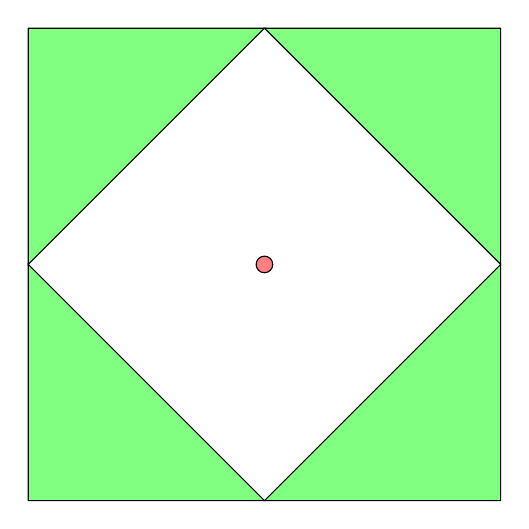
\begin{tikzpicture}
\draw (0,0)--(0,6)--(6,6)--(6,0)--(0,0);
\filldraw[fill=green!50!white] (0,0)--(0,3)--(3,0)--(0,0);
\filldraw[fill=green!50!white] (6,6)--(6,3)--(3,6)--(6,6);
\filldraw[fill=green!50!white] (0,6)--(0,3)--(3,6)--(0,6);
\filldraw[fill=green!50!white] (6,0)--(6,3)--(3,0)--(6,0);
\filldraw[fill=red!50!white] (3,3) circle (3pt);
\end{tikzpicture}
\end{figure}
اگر نقطه‌ی تصادفی مسئله، در یکی از نواحی سبز بیفتد، فاصله‌ی آن تا مرکز مربع از فاصله‌ی آن تا حداقل یکی از رئوس مربع بیشتر است. از آنجا که نواحی سبز، نصف مساحت مربع را اشغال می‌کنند در نتیجه احتمال مطلوب برابر 
$
\frac{1}{2}
$
خواهد بود.


\Q

الف) با قرار دادن رخ سفید، دقیقا 
$
2\times 8-2=14
$
خانه در معرض حمله‌ی رخ سفید قرار می‌گیرند (این موضوع، مستقل از مکان قرارگیری رخ سفید است). در نتیجه پیشامد مطلوب آن است که رخ سیاه، در یکی از این خانه‌ها قرار گیرد که این امر، با احتمال 
$
\frac{14}{63}=\frac{2}{9}
$
رخ می‌دهد.

ب) برای مات شدن شاه سفید، حتما باید حداقل یکی از رخ های سیاه، گوشه‌ای را که شاه سفید در آن قرار دارد تهدید کند. در نتیجه یکی از رخ ها باید در یکی از 14 خانه‌ی ممکن قرار داشته باشد. به دلیل تقارن مسئله، فرض می‌کنیم یک رخ سیاه، در پایینی ترین ردیف قرار دارد.

هنگامی که یک رخ، ردیف یا ستونی که شامل شاه است را تهدید می‌کند، برای مات کردن شاه، رخ دیگر باید ردیف یا ستون دیگری را که شاه می‌تواند حرکت کند، به طور کامل تهدید کند (شکل 2؛ دایره‌ی قرمز و مثل سبز به ترتیب نشان دهنده‌ی شاه سفید و رخ سیاه هستند). از طرفی، یکی از رخ ها نمی تواند خانه‌ی سیاه بالای شاه را اشغال کند؛ زیرا شاه با زدن آن مهره، از کیش و مات فرار میکند. همچنین اگر یکی از رخ‌ها در خانه‌ی مجاور شاه باشد، رخ دیگر نیز باید دقیقأ بالای آن قرار بگیرد و بالعکس؛ در غیر اینصورت، شاه با زدن رخ کنار خود یا رخی که در خانه‌ی همسایه‌ی قطری شاه قرار دارد، از کیش فرار می‌کند. در نتیجه، آرایش 2 تایی رخ ها به 
$
6\times 6+1=37
$
طریق ممکن امکان پذیر است. به دلیل تقارن، مات شدن می‌تواند به صورت ستونی نیز زخ دهد؛ در نتیجه تعداد کل حالات مطلوب برابر 
$
2\times 37=74
$
و احتمال مطلوب برابر 
$
\frac{74}{\binom{63}{2}}=\frac{74}{1953}
$
خواهد بود.

\begin{figure}[h]
\centering
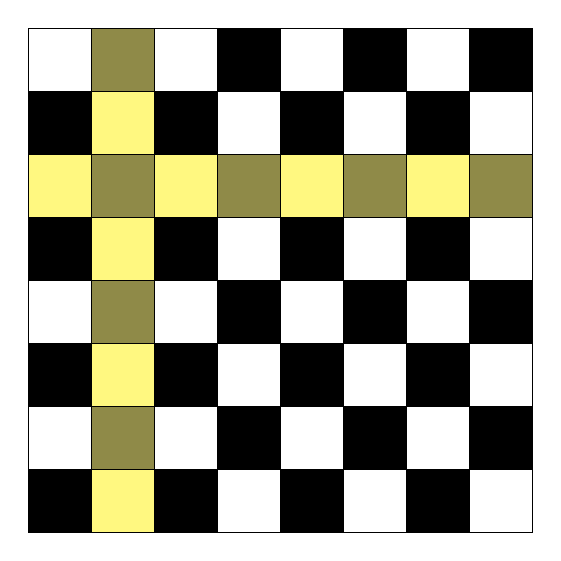
\begin{tikzpicture}
\filldraw[fill=black](-3.2,-3.2)--(-2.4000000000000004,-3.2)--(-2.4000000000000004,-2.4000000000000004)--(-3.2,-2.4000000000000004)--(-3.2,-3.2);
\filldraw[fill=white](-3.2,-2.4000000000000004)--(-2.4000000000000004,-2.4000000000000004)--(-2.4000000000000004,-1.6000000000000003)--(-3.2,-1.6000000000000003)--(-3.2,-2.4000000000000004);
\filldraw[fill=black](-3.2,-1.6)--(-2.4000000000000004,-1.6)--(-2.4000000000000004,-0.8)--(-3.2,-0.8)--(-3.2,-1.6);
\filldraw[fill=white](-3.2,-0.8)--(-2.4000000000000004,-0.8)--(-2.4000000000000004,0.0)--(-3.2,0.0)--(-3.2,-0.8);
\filldraw[fill=black](-3.2,0.0)--(-2.4000000000000004,0.0)--(-2.4000000000000004,0.8)--(-3.2,0.8)--(-3.2,0.0);
\filldraw[fill=yellow!50!white](-3.2,0.8)--(-2.4000000000000004,0.8)--(-2.4000000000000004,1.6)--(-3.2,1.6)--(-3.2,0.8);
\filldraw[fill=black](-3.2,1.6)--(-2.4000000000000004,1.6)--(-2.4000000000000004,2.4000000000000004)--(-3.2,2.4000000000000004)--(-3.2,1.6);
\filldraw[fill=white](-3.2,2.4000000000000004)--(-2.4000000000000004,2.4000000000000004)--(-2.4000000000000004,3.2)--(-3.2,3.2)--(-3.2,2.4000000000000004);
\filldraw[fill=yellow!50!white](-2.4000000000000004,-3.2)--(-1.6000000000000003,-3.2)--(-1.6000000000000003,-2.4000000000000004)--(-2.4000000000000004,-2.4000000000000004)--(-2.4000000000000004,-3.2);
\filldraw[fill=yellow!50!black](-2.4000000000000004,-2.4000000000000004)--(-1.6000000000000003,-2.4000000000000004)--(-1.6000000000000003,-1.6000000000000003)--(-2.4000000000000004,-1.6000000000000003)--(-2.4000000000000004,-2.4000000000000004);
\filldraw[fill=yellow!50!white](-2.4000000000000004,-1.6)--(-1.6000000000000003,-1.6)--(-1.6000000000000003,-0.8)--(-2.4000000000000004,-0.8)--(-2.4000000000000004,-1.6);
\filldraw[fill=yellow!50!black](-2.4000000000000004,-0.8)--(-1.6000000000000003,-0.8)--(-1.6000000000000003,0.0)--(-2.4000000000000004,0.0)--(-2.4000000000000004,-0.8);
\filldraw[fill=yellow!50!white](-2.4000000000000004,0.0)--(-1.6000000000000003,0.0)--(-1.6000000000000003,0.8)--(-2.4000000000000004,0.8)--(-2.4000000000000004,0.0);
\filldraw[fill=yellow!50!black](-2.4000000000000004,0.8)--(-1.6000000000000003,0.8)--(-1.6000000000000003,1.6)--(-2.4000000000000004,1.6)--(-2.4000000000000004,0.8);
\filldraw[fill=yellow!50!white](-2.4000000000000004,1.6)--(-1.6000000000000003,1.6)--(-1.6000000000000003,2.4000000000000004)--(-2.4000000000000004,2.4000000000000004)--(-2.4000000000000004,1.6);
\filldraw[fill=yellow!50!black](-2.4000000000000004,2.4000000000000004)--(-1.6000000000000003,2.4000000000000004)--(-1.6000000000000003,3.2)--(-2.4000000000000004,3.2)--(-2.4000000000000004,2.4000000000000004);
\filldraw[fill=black](-1.6,-3.2)--(-0.8,-3.2)--(-0.8,-2.4000000000000004)--(-1.6,-2.4000000000000004)--(-1.6,-3.2);
\filldraw[fill=white](-1.6,-2.4000000000000004)--(-0.8,-2.4000000000000004)--(-0.8,-1.6000000000000003)--(-1.6,-1.6000000000000003)--(-1.6,-2.4000000000000004);
\filldraw[fill=black](-1.6,-1.6)--(-0.8,-1.6)--(-0.8,-0.8)--(-1.6,-0.8)--(-1.6,-1.6);
\filldraw[fill=white](-1.6,-0.8)--(-0.8,-0.8)--(-0.8,0.0)--(-1.6,0.0)--(-1.6,-0.8);
\filldraw[fill=black](-1.6,0.0)--(-0.8,0.0)--(-0.8,0.8)--(-1.6,0.8)--(-1.6,0.0);
\filldraw[fill=yellow!50!white](-1.6,0.8)--(-0.8,0.8)--(-0.8,1.6)--(-1.6,1.6)--(-1.6,0.8);
\filldraw[fill=black](-1.6,1.6)--(-0.8,1.6)--(-0.8,2.4000000000000004)--(-1.6,2.4000000000000004)--(-1.6,1.6);
\filldraw[fill=white](-1.6,2.4000000000000004)--(-0.8,2.4000000000000004)--(-0.8,3.2)--(-1.6,3.2)--(-1.6,2.4000000000000004);
\filldraw[fill=white](-0.8,-3.2)--(0.0,-3.2)--(0.0,-2.4000000000000004)--(-0.8,-2.4000000000000004)--(-0.8,-3.2);
\filldraw[fill=black](-0.8,-2.4000000000000004)--(0.0,-2.4000000000000004)--(0.0,-1.6000000000000003)--(-0.8,-1.6000000000000003)--(-0.8,-2.4000000000000004);
\filldraw[fill=white](-0.8,-1.6)--(0.0,-1.6)--(0.0,-0.8)--(-0.8,-0.8)--(-0.8,-1.6);
\filldraw[fill=black](-0.8,-0.8)--(0.0,-0.8)--(0.0,0.0)--(-0.8,0.0)--(-0.8,-0.8);
\filldraw[fill=white](-0.8,0.0)--(0.0,0.0)--(0.0,0.8)--(-0.8,0.8)--(-0.8,0.0);
\filldraw[fill=yellow!50!black](-0.8,0.8)--(0.0,0.8)--(0.0,1.6)--(-0.8,1.6)--(-0.8,0.8);
\filldraw[fill=white](-0.8,1.6)--(0.0,1.6)--(0.0,2.4000000000000004)--(-0.8,2.4000000000000004)--(-0.8,1.6);
\filldraw[fill=black](-0.8,2.4000000000000004)--(0.0,2.4000000000000004)--(0.0,3.2)--(-0.8,3.2)--(-0.8,2.4000000000000004);
\filldraw[fill=black](0.0,-3.2)--(0.8,-3.2)--(0.8,-2.4000000000000004)--(0.0,-2.4000000000000004)--(0.0,-3.2);
\filldraw[fill=white](0.0,-2.4000000000000004)--(0.8,-2.4000000000000004)--(0.8,-1.6000000000000003)--(0.0,-1.6000000000000003)--(0.0,-2.4000000000000004);
\filldraw[fill=black](0.0,-1.6)--(0.8,-1.6)--(0.8,-0.8)--(0.0,-0.8)--(0.0,-1.6);
\filldraw[fill=white](0.0,-0.8)--(0.8,-0.8)--(0.8,0.0)--(0.0,0.0)--(0.0,-0.8);
\filldraw[fill=black](0.0,0.0)--(0.8,0.0)--(0.8,0.8)--(0.0,0.8)--(0.0,0.0);
\filldraw[fill=yellow!50!white](0.0,0.8)--(0.8,0.8)--(0.8,1.6)--(0.0,1.6)--(0.0,0.8);
\filldraw[fill=black](0.0,1.6)--(0.8,1.6)--(0.8,2.4000000000000004)--(0.0,2.4000000000000004)--(0.0,1.6);
\filldraw[fill=white](0.0,2.4000000000000004)--(0.8,2.4000000000000004)--(0.8,3.2)--(0.0,3.2)--(0.0,2.4000000000000004);
\filldraw[fill=white](0.8,-3.2)--(1.6,-3.2)--(1.6,-2.4000000000000004)--(0.8,-2.4000000000000004)--(0.8,-3.2);
\filldraw[fill=black](0.8,-2.4000000000000004)--(1.6,-2.4000000000000004)--(1.6,-1.6000000000000003)--(0.8,-1.6000000000000003)--(0.8,-2.4000000000000004);
\filldraw[fill=white](0.8,-1.6)--(1.6,-1.6)--(1.6,-0.8)--(0.8,-0.8)--(0.8,-1.6);
\filldraw[fill=black](0.8,-0.8)--(1.6,-0.8)--(1.6,0.0)--(0.8,0.0)--(0.8,-0.8);
\filldraw[fill=white](0.8,0.0)--(1.6,0.0)--(1.6,0.8)--(0.8,0.8)--(0.8,0.0);
\filldraw[fill=yellow!50!black](0.8,0.8)--(1.6,0.8)--(1.6,1.6)--(0.8,1.6)--(0.8,0.8);
\filldraw[fill=white](0.8,1.6)--(1.6,1.6)--(1.6,2.4000000000000004)--(0.8,2.4000000000000004)--(0.8,1.6);
\filldraw[fill=black](0.8,2.4000000000000004)--(1.6,2.4000000000000004)--(1.6,3.2)--(0.8,3.2)--(0.8,2.4000000000000004);
\filldraw[fill=black](1.6,-3.2)--(2.4000000000000004,-3.2)--(2.4000000000000004,-2.4000000000000004)--(1.6,-2.4000000000000004)--(1.6,-3.2);
\filldraw[fill=white](1.6,-2.4000000000000004)--(2.4000000000000004,-2.4000000000000004)--(2.4000000000000004,-1.6000000000000003)--(1.6,-1.6000000000000003)--(1.6,-2.4000000000000004);
\filldraw[fill=black](1.6,-1.6)--(2.4000000000000004,-1.6)--(2.4000000000000004,-0.8)--(1.6,-0.8)--(1.6,-1.6);
\filldraw[fill=white](1.6,-0.8)--(2.4000000000000004,-0.8)--(2.4000000000000004,0.0)--(1.6,0.0)--(1.6,-0.8);
\filldraw[fill=black](1.6,0.0)--(2.4000000000000004,0.0)--(2.4000000000000004,0.8)--(1.6,0.8)--(1.6,0.0);
\filldraw[fill=yellow!50!white](1.6,0.8)--(2.4000000000000004,0.8)--(2.4000000000000004,1.6)--(1.6,1.6)--(1.6,0.8);
\filldraw[fill=black](1.6,1.6)--(2.4000000000000004,1.6)--(2.4000000000000004,2.4000000000000004)--(1.6,2.4000000000000004)--(1.6,1.6);
\filldraw[fill=white](1.6,2.4000000000000004)--(2.4000000000000004,2.4000000000000004)--(2.4000000000000004,3.2)--(1.6,3.2)--(1.6,2.4000000000000004);
\filldraw[fill=white](2.4000000000000004,-3.2)--(3.2,-3.2)--(3.2,-2.4000000000000004)--(2.4000000000000004,-2.4000000000000004)--(2.4000000000000004,-3.2);
\filldraw[fill=black](2.4000000000000004,-2.4000000000000004)--(3.2,-2.4000000000000004)--(3.2,-1.6000000000000003)--(2.4000000000000004,-1.6000000000000003)--(2.4000000000000004,-2.4000000000000004);
\filldraw[fill=white](2.4000000000000004,-1.6)--(3.2,-1.6)--(3.2,-0.8)--(2.4000000000000004,-0.8)--(2.4000000000000004,-1.6);
\filldraw[fill=black](2.4000000000000004,-0.8)--(3.2,-0.8)--(3.2,0.0)--(2.4000000000000004,0.0)--(2.4000000000000004,-0.8);
\filldraw[fill=white](2.4000000000000004,0.0)--(3.2,0.0)--(3.2,0.8)--(2.4000000000000004,0.8)--(2.4000000000000004,0.0);
\filldraw[fill=yellow!50!black](2.4000000000000004,0.8)--(3.2,0.8)--(3.2,1.6)--(2.4000000000000004,1.6)--(2.4000000000000004,0.8);
\filldraw[fill=white](2.4000000000000004,1.6)--(3.2,1.6)--(3.2,2.4000000000000004)--(2.4000000000000004,2.4000000000000004)--(2.4000000000000004,1.6);
\filldraw[fill=black](2.4000000000000004,2.4000000000000004)--(3.2,2.4000000000000004)--(3.2,3.2)--(2.4000000000000004,3.2)--(2.4000000000000004,2.4000000000000004);
\end{tikzpicture}
\vspace{10mm}
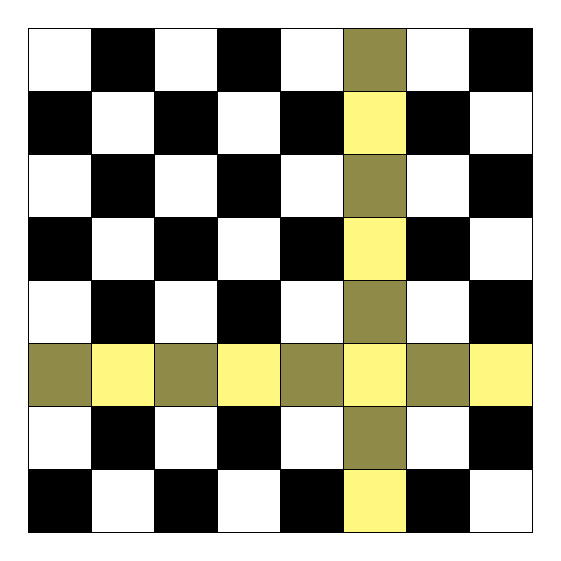
\begin{tikzpicture}
\filldraw[fill=black](-3.2,-3.2)--(-2.4000000000000004,-3.2)--(-2.4000000000000004,-2.4000000000000004)--(-3.2,-2.4000000000000004)--(-3.2,-3.2);
\filldraw[fill=white](-3.2,-2.4000000000000004)--(-2.4000000000000004,-2.4000000000000004)--(-2.4000000000000004,-1.6000000000000003)--(-3.2,-1.6000000000000003)--(-3.2,-2.4000000000000004);
\filldraw[fill=yellow!50!black](-3.2,-1.6)--(-2.4000000000000004,-1.6)--(-2.4000000000000004,-0.8)--(-3.2,-0.8)--(-3.2,-1.6);
\filldraw[fill=white](-3.2,-0.8)--(-2.4000000000000004,-0.8)--(-2.4000000000000004,0.0)--(-3.2,0.0)--(-3.2,-0.8);
\filldraw[fill=black](-3.2,0.0)--(-2.4000000000000004,0.0)--(-2.4000000000000004,0.8)--(-3.2,0.8)--(-3.2,0.0);
\filldraw[fill=white](-3.2,0.8)--(-2.4000000000000004,0.8)--(-2.4000000000000004,1.6)--(-3.2,1.6)--(-3.2,0.8);
\filldraw[fill=black](-3.2,1.6)--(-2.4000000000000004,1.6)--(-2.4000000000000004,2.4000000000000004)--(-3.2,2.4000000000000004)--(-3.2,1.6);
\filldraw[fill=white](-3.2,2.4000000000000004)--(-2.4000000000000004,2.4000000000000004)--(-2.4000000000000004,3.2)--(-3.2,3.2)--(-3.2,2.4000000000000004);
\filldraw[fill=white](-2.4000000000000004,-3.2)--(-1.6000000000000003,-3.2)--(-1.6000000000000003,-2.4000000000000004)--(-2.4000000000000004,-2.4000000000000004)--(-2.4000000000000004,-3.2);
\filldraw[fill=black](-2.4000000000000004,-2.4000000000000004)--(-1.6000000000000003,-2.4000000000000004)--(-1.6000000000000003,-1.6000000000000003)--(-2.4000000000000004,-1.6000000000000003)--(-2.4000000000000004,-2.4000000000000004);
\filldraw[fill=yellow!50!white](-2.4000000000000004,-1.6)--(-1.6000000000000003,-1.6)--(-1.6000000000000003,-0.8)--(-2.4000000000000004,-0.8)--(-2.4000000000000004,-1.6);
\filldraw[fill=black](-2.4000000000000004,-0.8)--(-1.6000000000000003,-0.8)--(-1.6000000000000003,0.0)--(-2.4000000000000004,0.0)--(-2.4000000000000004,-0.8);
\filldraw[fill=white](-2.4000000000000004,0.0)--(-1.6000000000000003,0.0)--(-1.6000000000000003,0.8)--(-2.4000000000000004,0.8)--(-2.4000000000000004,0.0);
\filldraw[fill=black](-2.4000000000000004,0.8)--(-1.6000000000000003,0.8)--(-1.6000000000000003,1.6)--(-2.4000000000000004,1.6)--(-2.4000000000000004,0.8);
\filldraw[fill=white](-2.4000000000000004,1.6)--(-1.6000000000000003,1.6)--(-1.6000000000000003,2.4000000000000004)--(-2.4000000000000004,2.4000000000000004)--(-2.4000000000000004,1.6);
\filldraw[fill=black](-2.4000000000000004,2.4000000000000004)--(-1.6000000000000003,2.4000000000000004)--(-1.6000000000000003,3.2)--(-2.4000000000000004,3.2)--(-2.4000000000000004,2.4000000000000004);
\filldraw[fill=black](-1.6,-3.2)--(-0.8,-3.2)--(-0.8,-2.4000000000000004)--(-1.6,-2.4000000000000004)--(-1.6,-3.2);
\filldraw[fill=white](-1.6,-2.4000000000000004)--(-0.8,-2.4000000000000004)--(-0.8,-1.6000000000000003)--(-1.6,-1.6000000000000003)--(-1.6,-2.4000000000000004);
\filldraw[fill=yellow!50!black](-1.6,-1.6)--(-0.8,-1.6)--(-0.8,-0.8)--(-1.6,-0.8)--(-1.6,-1.6);
\filldraw[fill=white](-1.6,-0.8)--(-0.8,-0.8)--(-0.8,0.0)--(-1.6,0.0)--(-1.6,-0.8);
\filldraw[fill=black](-1.6,0.0)--(-0.8,0.0)--(-0.8,0.8)--(-1.6,0.8)--(-1.6,0.0);
\filldraw[fill=white](-1.6,0.8)--(-0.8,0.8)--(-0.8,1.6)--(-1.6,1.6)--(-1.6,0.8);
\filldraw[fill=black](-1.6,1.6)--(-0.8,1.6)--(-0.8,2.4000000000000004)--(-1.6,2.4000000000000004)--(-1.6,1.6);
\filldraw[fill=white](-1.6,2.4000000000000004)--(-0.8,2.4000000000000004)--(-0.8,3.2)--(-1.6,3.2)--(-1.6,2.4000000000000004);
\filldraw[fill=white](-0.8,-3.2)--(0.0,-3.2)--(0.0,-2.4000000000000004)--(-0.8,-2.4000000000000004)--(-0.8,-3.2);
\filldraw[fill=black](-0.8,-2.4000000000000004)--(0.0,-2.4000000000000004)--(0.0,-1.6000000000000003)--(-0.8,-1.6000000000000003)--(-0.8,-2.4000000000000004);
\filldraw[fill=yellow!50!white](-0.8,-1.6)--(0.0,-1.6)--(0.0,-0.8)--(-0.8,-0.8)--(-0.8,-1.6);
\filldraw[fill=black](-0.8,-0.8)--(0.0,-0.8)--(0.0,0.0)--(-0.8,0.0)--(-0.8,-0.8);
\filldraw[fill=white](-0.8,0.0)--(0.0,0.0)--(0.0,0.8)--(-0.8,0.8)--(-0.8,0.0);
\filldraw[fill=black](-0.8,0.8)--(0.0,0.8)--(0.0,1.6)--(-0.8,1.6)--(-0.8,0.8);
\filldraw[fill=white](-0.8,1.6)--(0.0,1.6)--(0.0,2.4000000000000004)--(-0.8,2.4000000000000004)--(-0.8,1.6);
\filldraw[fill=black](-0.8,2.4000000000000004)--(0.0,2.4000000000000004)--(0.0,3.2)--(-0.8,3.2)--(-0.8,2.4000000000000004);
\filldraw[fill=black](0.0,-3.2)--(0.8,-3.2)--(0.8,-2.4000000000000004)--(0.0,-2.4000000000000004)--(0.0,-3.2);
\filldraw[fill=white](0.0,-2.4000000000000004)--(0.8,-2.4000000000000004)--(0.8,-1.6000000000000003)--(0.0,-1.6000000000000003)--(0.0,-2.4000000000000004);
\filldraw[fill=yellow!50!black](0.0,-1.6)--(0.8,-1.6)--(0.8,-0.8)--(0.0,-0.8)--(0.0,-1.6);
\filldraw[fill=white](0.0,-0.8)--(0.8,-0.8)--(0.8,0.0)--(0.0,0.0)--(0.0,-0.8);
\filldraw[fill=black](0.0,0.0)--(0.8,0.0)--(0.8,0.8)--(0.0,0.8)--(0.0,0.0);
\filldraw[fill=white](0.0,0.8)--(0.8,0.8)--(0.8,1.6)--(0.0,1.6)--(0.0,0.8);
\filldraw[fill=black](0.0,1.6)--(0.8,1.6)--(0.8,2.4000000000000004)--(0.0,2.4000000000000004)--(0.0,1.6);
\filldraw[fill=white](0.0,2.4000000000000004)--(0.8,2.4000000000000004)--(0.8,3.2)--(0.0,3.2)--(0.0,2.4000000000000004);
\filldraw[fill=yellow!50!white](0.8,-3.2)--(1.6,-3.2)--(1.6,-2.4000000000000004)--(0.8,-2.4000000000000004)--(0.8,-3.2);
\filldraw[fill=yellow!50!black](0.8,-2.4000000000000004)--(1.6,-2.4000000000000004)--(1.6,-1.6000000000000003)--(0.8,-1.6000000000000003)--(0.8,-2.4000000000000004);
\filldraw[fill=yellow!50!white](0.8,-1.6)--(1.6,-1.6)--(1.6,-0.8)--(0.8,-0.8)--(0.8,-1.6);
\filldraw[fill=yellow!50!black](0.8,-0.8)--(1.6,-0.8)--(1.6,0.0)--(0.8,0.0)--(0.8,-0.8);
\filldraw[fill=yellow!50!white](0.8,0.0)--(1.6,0.0)--(1.6,0.8)--(0.8,0.8)--(0.8,0.0);
\filldraw[fill=yellow!50!black](0.8,0.8)--(1.6,0.8)--(1.6,1.6)--(0.8,1.6)--(0.8,0.8);
\filldraw[fill=yellow!50!white](0.8,1.6)--(1.6,1.6)--(1.6,2.4000000000000004)--(0.8,2.4000000000000004)--(0.8,1.6);
\filldraw[fill=yellow!50!black](0.8,2.4000000000000004)--(1.6,2.4000000000000004)--(1.6,3.2)--(0.8,3.2)--(0.8,2.4000000000000004);
\filldraw[fill=black](1.6,-3.2)--(2.4000000000000004,-3.2)--(2.4000000000000004,-2.4000000000000004)--(1.6,-2.4000000000000004)--(1.6,-3.2);
\filldraw[fill=white](1.6,-2.4000000000000004)--(2.4000000000000004,-2.4000000000000004)--(2.4000000000000004,-1.6000000000000003)--(1.6,-1.6000000000000003)--(1.6,-2.4000000000000004);
\filldraw[fill=yellow!50!black](1.6,-1.6)--(2.4000000000000004,-1.6)--(2.4000000000000004,-0.8)--(1.6,-0.8)--(1.6,-1.6);
\filldraw[fill=white](1.6,-0.8)--(2.4000000000000004,-0.8)--(2.4000000000000004,0.0)--(1.6,0.0)--(1.6,-0.8);
\filldraw[fill=black](1.6,0.0)--(2.4000000000000004,0.0)--(2.4000000000000004,0.8)--(1.6,0.8)--(1.6,0.0);
\filldraw[fill=white](1.6,0.8)--(2.4000000000000004,0.8)--(2.4000000000000004,1.6)--(1.6,1.6)--(1.6,0.8);
\filldraw[fill=black](1.6,1.6)--(2.4000000000000004,1.6)--(2.4000000000000004,2.4000000000000004)--(1.6,2.4000000000000004)--(1.6,1.6);
\filldraw[fill=white](1.6,2.4000000000000004)--(2.4000000000000004,2.4000000000000004)--(2.4000000000000004,3.2)--(1.6,3.2)--(1.6,2.4000000000000004);
\filldraw[fill=white](2.4000000000000004,-3.2)--(3.2,-3.2)--(3.2,-2.4000000000000004)--(2.4000000000000004,-2.4000000000000004)--(2.4000000000000004,-3.2);
\filldraw[fill=black](2.4000000000000004,-2.4000000000000004)--(3.2,-2.4000000000000004)--(3.2,-1.6000000000000003)--(2.4000000000000004,-1.6000000000000003)--(2.4000000000000004,-2.4000000000000004);
\filldraw[fill=yellow!50!white](2.4000000000000004,-1.6)--(3.2,-1.6)--(3.2,-0.8)--(2.4000000000000004,-0.8)--(2.4000000000000004,-1.6);
\filldraw[fill=black](2.4000000000000004,-0.8)--(3.2,-0.8)--(3.2,0.0)--(2.4000000000000004,0.0)--(2.4000000000000004,-0.8);
\filldraw[fill=white](2.4000000000000004,0.0)--(3.2,0.0)--(3.2,0.8)--(2.4000000000000004,0.8)--(2.4000000000000004,0.0);
\filldraw[fill=black](2.4000000000000004,0.8)--(3.2,0.8)--(3.2,1.6)--(2.4000000000000004,1.6)--(2.4000000000000004,0.8);
\filldraw[fill=white](2.4000000000000004,1.6)--(3.2,1.6)--(3.2,2.4000000000000004)--(2.4000000000000004,2.4000000000000004)--(2.4000000000000004,1.6);
\filldraw[fill=black](2.4000000000000004,2.4000000000000004)--(3.2,2.4000000000000004)--(3.2,3.2)--(2.4000000000000004,3.2)--(2.4000000000000004,2.4000000000000004);
\end{tikzpicture}
\caption{
دو نمودار مربوط به سوال 2 قسمت الف
}
\end{figure}

\begin{figure}[h]
\centering
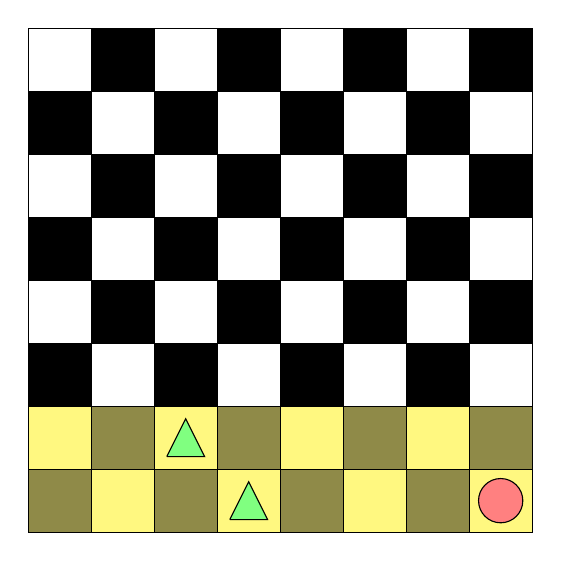
\begin{tikzpicture}
\filldraw[fill=yellow!50!black](0.8,0.8)--(1.6,0.8)--(1.6,1.6)--(0.8,1.6)--(0.8,0.8);
\filldraw[fill=yellow!50!white](0.8,1.6)--(1.6,1.6)--(1.6,2.4000000000000004)--(0.8,2.4000000000000004)--(0.8,1.6);
\filldraw[fill=black](0.8,2.4000000000000004)--(1.6,2.4000000000000004)--(1.6,3.2)--(0.8,3.2)--(0.8,2.4000000000000004);
\filldraw[fill=white](0.8,3.2)--(1.6,3.2)--(1.6,4.0)--(0.8,4.0)--(0.8,3.2);
\filldraw[fill=black](0.8,4.0)--(1.6,4.0)--(1.6,4.8)--(0.8,4.8)--(0.8,4.0);
\filldraw[fill=white](0.8,4.800000000000001)--(1.6,4.800000000000001)--(1.6,5.6000000000000005)--(0.8,5.6000000000000005)--(0.8,4.800000000000001);
\filldraw[fill=black](0.8,5.6000000000000005)--(1.6,5.6000000000000005)--(1.6,6.4)--(0.8,6.4)--(0.8,5.6000000000000005);
\filldraw[fill=white](0.8,6.4)--(1.6,6.4)--(1.6,7.2)--(0.8,7.2)--(0.8,6.4);
\filldraw[fill=yellow!50!white](1.6,0.8)--(2.4000000000000004,0.8)--(2.4000000000000004,1.6)--(1.6,1.6)--(1.6,0.8);
\filldraw[fill=yellow!50!black](1.6,1.6)--(2.4000000000000004,1.6)--(2.4000000000000004,2.4000000000000004)--(1.6,2.4000000000000004)--(1.6,1.6);
\filldraw[fill=white](1.6,2.4000000000000004)--(2.4000000000000004,2.4000000000000004)--(2.4000000000000004,3.2)--(1.6,3.2)--(1.6,2.4000000000000004);
\filldraw[fill=black](1.6,3.2)--(2.4000000000000004,3.2)--(2.4000000000000004,4.0)--(1.6,4.0)--(1.6,3.2);
\filldraw[fill=white](1.6,4.0)--(2.4000000000000004,4.0)--(2.4000000000000004,4.8)--(1.6,4.8)--(1.6,4.0);
\filldraw[fill=black](1.6,4.800000000000001)--(2.4000000000000004,4.800000000000001)--(2.4000000000000004,5.6000000000000005)--(1.6,5.6000000000000005)--(1.6,4.800000000000001);
\filldraw[fill=white](1.6,5.6000000000000005)--(2.4000000000000004,5.6000000000000005)--(2.4000000000000004,6.4)--(1.6,6.4)--(1.6,5.6000000000000005);
\filldraw[fill=black](1.6,6.4)--(2.4000000000000004,6.4)--(2.4000000000000004,7.2)--(1.6,7.2)--(1.6,6.4);
\filldraw[fill=yellow!50!black](2.4000000000000004,0.8)--(3.2,0.8)--(3.2,1.6)--(2.4000000000000004,1.6)--(2.4000000000000004,0.8);
\filldraw[fill=yellow!50!white](2.4000000000000004,1.6)--(3.2,1.6)--(3.2,2.4000000000000004)--(2.4000000000000004,2.4000000000000004)--(2.4000000000000004,1.6);
\filldraw[fill=green!50!white] (2.5600000000000005,1.7600000000000002)--(3.04,1.7600000000000002)--(2.8000000000000003,2.2399999999999998)--(2.5600000000000005,1.7600000000000002);
\filldraw[fill=black](2.4000000000000004,2.4000000000000004)--(3.2,2.4000000000000004)--(3.2,3.2)--(2.4000000000000004,3.2)--(2.4000000000000004,2.4000000000000004);
\filldraw[fill=white](2.4000000000000004,3.2)--(3.2,3.2)--(3.2,4.0)--(2.4000000000000004,4.0)--(2.4000000000000004,3.2);
\filldraw[fill=black](2.4000000000000004,4.0)--(3.2,4.0)--(3.2,4.8)--(2.4000000000000004,4.8)--(2.4000000000000004,4.0);
\filldraw[fill=white](2.4000000000000004,4.800000000000001)--(3.2,4.800000000000001)--(3.2,5.6000000000000005)--(2.4000000000000004,5.6000000000000005)--(2.4000000000000004,4.800000000000001);
\filldraw[fill=black](2.4000000000000004,5.6000000000000005)--(3.2,5.6000000000000005)--(3.2,6.4)--(2.4000000000000004,6.4)--(2.4000000000000004,5.6000000000000005);
\filldraw[fill=white](2.4000000000000004,6.4)--(3.2,6.4)--(3.2,7.2)--(2.4000000000000004,7.2)--(2.4000000000000004,6.4);
\filldraw[fill=yellow!50!white](3.2,0.8)--(4.0,0.8)--(4.0,1.6)--(3.2,1.6)--(3.2,0.8);
\filldraw[fill=green!50!white] (3.3600000000000003,0.96)--(3.84,0.96)--(3.6,1.4400000000000002)--(3.3600000000000003,0.96);
\filldraw[fill=yellow!50!black](3.2,1.6)--(4.0,1.6)--(4.0,2.4000000000000004)--(3.2,2.4000000000000004)--(3.2,1.6);
\filldraw[fill=white](3.2,2.4000000000000004)--(4.0,2.4000000000000004)--(4.0,3.2)--(3.2,3.2)--(3.2,2.4000000000000004);
\filldraw[fill=black](3.2,3.2)--(4.0,3.2)--(4.0,4.0)--(3.2,4.0)--(3.2,3.2);
\filldraw[fill=white](3.2,4.0)--(4.0,4.0)--(4.0,4.8)--(3.2,4.8)--(3.2,4.0);
\filldraw[fill=black](3.2,4.800000000000001)--(4.0,4.800000000000001)--(4.0,5.6000000000000005)--(3.2,5.6000000000000005)--(3.2,4.800000000000001);
\filldraw[fill=white](3.2,5.6000000000000005)--(4.0,5.6000000000000005)--(4.0,6.4)--(3.2,6.4)--(3.2,5.6000000000000005);
\filldraw[fill=black](3.2,6.4)--(4.0,6.4)--(4.0,7.2)--(3.2,7.2)--(3.2,6.4);
\filldraw[fill=yellow!50!black](4.0,0.8)--(4.8,0.8)--(4.8,1.6)--(4.0,1.6)--(4.0,0.8);
\filldraw[fill=yellow!50!white](4.0,1.6)--(4.8,1.6)--(4.8,2.4000000000000004)--(4.0,2.4000000000000004)--(4.0,1.6);
\filldraw[fill=black](4.0,2.4000000000000004)--(4.8,2.4000000000000004)--(4.8,3.2)--(4.0,3.2)--(4.0,2.4000000000000004);
\filldraw[fill=white](4.0,3.2)--(4.8,3.2)--(4.8,4.0)--(4.0,4.0)--(4.0,3.2);
\filldraw[fill=black](4.0,4.0)--(4.8,4.0)--(4.8,4.8)--(4.0,4.8)--(4.0,4.0);
\filldraw[fill=white](4.0,4.800000000000001)--(4.8,4.800000000000001)--(4.8,5.6000000000000005)--(4.0,5.6000000000000005)--(4.0,4.800000000000001);
\filldraw[fill=black](4.0,5.6000000000000005)--(4.8,5.6000000000000005)--(4.8,6.4)--(4.0,6.4)--(4.0,5.6000000000000005);
\filldraw[fill=white](4.0,6.4)--(4.8,6.4)--(4.8,7.2)--(4.0,7.2)--(4.0,6.4);
\filldraw[fill=yellow!50!white](4.800000000000001,0.8)--(5.6000000000000005,0.8)--(5.6000000000000005,1.6)--(4.800000000000001,1.6)--(4.800000000000001,0.8);
\filldraw[fill=yellow!50!black](4.800000000000001,1.6)--(5.6000000000000005,1.6)--(5.6000000000000005,2.4000000000000004)--(4.800000000000001,2.4000000000000004)--(4.800000000000001,1.6);
\filldraw[fill=white](4.800000000000001,2.4000000000000004)--(5.6000000000000005,2.4000000000000004)--(5.6000000000000005,3.2)--(4.800000000000001,3.2)--(4.800000000000001,2.4000000000000004);
\filldraw[fill=black](4.800000000000001,3.2)--(5.6000000000000005,3.2)--(5.6000000000000005,4.0)--(4.800000000000001,4.0)--(4.800000000000001,3.2);
\filldraw[fill=white](4.800000000000001,4.0)--(5.6000000000000005,4.0)--(5.6000000000000005,4.8)--(4.800000000000001,4.8)--(4.800000000000001,4.0);
\filldraw[fill=black](4.800000000000001,4.800000000000001)--(5.6000000000000005,4.800000000000001)--(5.6000000000000005,5.6000000000000005)--(4.800000000000001,5.6000000000000005)--(4.800000000000001,4.800000000000001);
\filldraw[fill=white](4.800000000000001,5.6000000000000005)--(5.6000000000000005,5.6000000000000005)--(5.6000000000000005,6.4)--(4.800000000000001,6.4)--(4.800000000000001,5.6000000000000005);
\filldraw[fill=black](4.800000000000001,6.4)--(5.6000000000000005,6.4)--(5.6000000000000005,7.2)--(4.800000000000001,7.2)--(4.800000000000001,6.4);
\filldraw[fill=yellow!50!black](5.6000000000000005,0.8)--(6.4,0.8)--(6.4,1.6)--(5.6000000000000005,1.6)--(5.6000000000000005,0.8);
\filldraw[fill=yellow!50!white](5.6000000000000005,1.6)--(6.4,1.6)--(6.4,2.4000000000000004)--(5.6000000000000005,2.4000000000000004)--(5.6000000000000005,1.6);
\filldraw[fill=black](5.6000000000000005,2.4000000000000004)--(6.4,2.4000000000000004)--(6.4,3.2)--(5.6000000000000005,3.2)--(5.6000000000000005,2.4000000000000004);
\filldraw[fill=white](5.6000000000000005,3.2)--(6.4,3.2)--(6.4,4.0)--(5.6000000000000005,4.0)--(5.6000000000000005,3.2);
\filldraw[fill=black](5.6000000000000005,4.0)--(6.4,4.0)--(6.4,4.8)--(5.6000000000000005,4.8)--(5.6000000000000005,4.0);
\filldraw[fill=white](5.6000000000000005,4.800000000000001)--(6.4,4.800000000000001)--(6.4,5.6000000000000005)--(5.6000000000000005,5.6000000000000005)--(5.6000000000000005,4.800000000000001);
\filldraw[fill=black](5.6000000000000005,5.6000000000000005)--(6.4,5.6000000000000005)--(6.4,6.4)--(5.6000000000000005,6.4)--(5.6000000000000005,5.6000000000000005);
\filldraw[fill=white](5.6000000000000005,6.4)--(6.4,6.4)--(6.4,7.2)--(5.6000000000000005,7.2)--(5.6000000000000005,6.4);
\filldraw[fill=yellow!50!white](6.4,0.8)--(7.2,0.8)--(7.2,1.6)--(6.4,1.6)--(6.4,0.8);
\filldraw[fill=red!50!white] (6.800000000000001,1.2000000000000002) circle (8pt);
\filldraw[fill=yellow!50!black](6.4,1.6)--(7.2,1.6)--(7.2,2.4000000000000004)--(6.4,2.4000000000000004)--(6.4,1.6);
\filldraw[fill=white](6.4,2.4000000000000004)--(7.2,2.4000000000000004)--(7.2,3.2)--(6.4,3.2)--(6.4,2.4000000000000004);
\filldraw[fill=black](6.4,3.2)--(7.2,3.2)--(7.2,4.0)--(6.4,4.0)--(6.4,3.2);
\filldraw[fill=white](6.4,4.0)--(7.2,4.0)--(7.2,4.8)--(6.4,4.8)--(6.4,4.0);
\filldraw[fill=black](6.4,4.800000000000001)--(7.2,4.800000000000001)--(7.2,5.6000000000000005)--(6.4,5.6000000000000005)--(6.4,4.800000000000001);
\filldraw[fill=white](6.4,5.6000000000000005)--(7.2,5.6000000000000005)--(7.2,6.4)--(6.4,6.4)--(6.4,5.6000000000000005);
\filldraw[fill=black](6.4,6.4)--(7.2,6.4)--(7.2,7.2)--(6.4,7.2)--(6.4,6.4);
\end{tikzpicture}
\caption{
مثالی از مات شدن شاه سفید
}
\end{figure}

\begin{figure}[h]
\centering
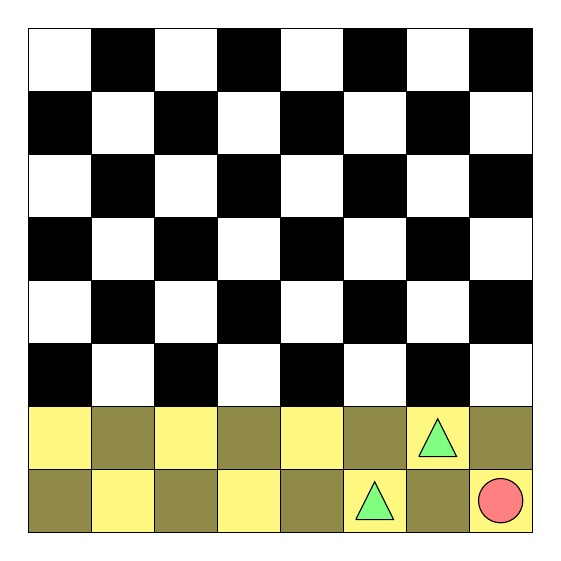
\begin{tikzpicture}
\filldraw[fill=yellow!50!black](0.8,0.8)--(1.6,0.8)--(1.6,1.6)--(0.8,1.6)--(0.8,0.8);
\filldraw[fill=yellow!50!white](0.8,1.6)--(1.6,1.6)--(1.6,2.4000000000000004)--(0.8,2.4000000000000004)--(0.8,1.6);
\filldraw[fill=black](0.8,2.4000000000000004)--(1.6,2.4000000000000004)--(1.6,3.2)--(0.8,3.2)--(0.8,2.4000000000000004);
\filldraw[fill=white](0.8,3.2)--(1.6,3.2)--(1.6,4.0)--(0.8,4.0)--(0.8,3.2);
\filldraw[fill=black](0.8,4.0)--(1.6,4.0)--(1.6,4.8)--(0.8,4.8)--(0.8,4.0);
\filldraw[fill=white](0.8,4.800000000000001)--(1.6,4.800000000000001)--(1.6,5.6000000000000005)--(0.8,5.6000000000000005)--(0.8,4.800000000000001);
\filldraw[fill=black](0.8,5.6000000000000005)--(1.6,5.6000000000000005)--(1.6,6.4)--(0.8,6.4)--(0.8,5.6000000000000005);
\filldraw[fill=white](0.8,6.4)--(1.6,6.4)--(1.6,7.2)--(0.8,7.2)--(0.8,6.4);
\filldraw[fill=yellow!50!white](1.6,0.8)--(2.4000000000000004,0.8)--(2.4000000000000004,1.6)--(1.6,1.6)--(1.6,0.8);
\filldraw[fill=yellow!50!black](1.6,1.6)--(2.4000000000000004,1.6)--(2.4000000000000004,2.4000000000000004)--(1.6,2.4000000000000004)--(1.6,1.6);
\filldraw[fill=white](1.6,2.4000000000000004)--(2.4000000000000004,2.4000000000000004)--(2.4000000000000004,3.2)--(1.6,3.2)--(1.6,2.4000000000000004);
\filldraw[fill=black](1.6,3.2)--(2.4000000000000004,3.2)--(2.4000000000000004,4.0)--(1.6,4.0)--(1.6,3.2);
\filldraw[fill=white](1.6,4.0)--(2.4000000000000004,4.0)--(2.4000000000000004,4.8)--(1.6,4.8)--(1.6,4.0);
\filldraw[fill=black](1.6,4.800000000000001)--(2.4000000000000004,4.800000000000001)--(2.4000000000000004,5.6000000000000005)--(1.6,5.6000000000000005)--(1.6,4.800000000000001);
\filldraw[fill=white](1.6,5.6000000000000005)--(2.4000000000000004,5.6000000000000005)--(2.4000000000000004,6.4)--(1.6,6.4)--(1.6,5.6000000000000005);
\filldraw[fill=black](1.6,6.4)--(2.4000000000000004,6.4)--(2.4000000000000004,7.2)--(1.6,7.2)--(1.6,6.4);
\filldraw[fill=yellow!50!black](2.4000000000000004,0.8)--(3.2,0.8)--(3.2,1.6)--(2.4000000000000004,1.6)--(2.4000000000000004,0.8);
\filldraw[fill=yellow!50!white](2.4000000000000004,1.6)--(3.2,1.6)--(3.2,2.4000000000000004)--(2.4000000000000004,2.4000000000000004)--(2.4000000000000004,1.6);
\filldraw[fill=black](2.4000000000000004,2.4000000000000004)--(3.2,2.4000000000000004)--(3.2,3.2)--(2.4000000000000004,3.2)--(2.4000000000000004,2.4000000000000004);
\filldraw[fill=white](2.4000000000000004,3.2)--(3.2,3.2)--(3.2,4.0)--(2.4000000000000004,4.0)--(2.4000000000000004,3.2);
\filldraw[fill=black](2.4000000000000004,4.0)--(3.2,4.0)--(3.2,4.8)--(2.4000000000000004,4.8)--(2.4000000000000004,4.0);
\filldraw[fill=white](2.4000000000000004,4.800000000000001)--(3.2,4.800000000000001)--(3.2,5.6000000000000005)--(2.4000000000000004,5.6000000000000005)--(2.4000000000000004,4.800000000000001);
\filldraw[fill=black](2.4000000000000004,5.6000000000000005)--(3.2,5.6000000000000005)--(3.2,6.4)--(2.4000000000000004,6.4)--(2.4000000000000004,5.6000000000000005);
\filldraw[fill=white](2.4000000000000004,6.4)--(3.2,6.4)--(3.2,7.2)--(2.4000000000000004,7.2)--(2.4000000000000004,6.4);
\filldraw[fill=yellow!50!white](3.2,0.8)--(4.0,0.8)--(4.0,1.6)--(3.2,1.6)--(3.2,0.8);
\filldraw[fill=yellow!50!black](3.2,1.6)--(4.0,1.6)--(4.0,2.4000000000000004)--(3.2,2.4000000000000004)--(3.2,1.6);
\filldraw[fill=white](3.2,2.4000000000000004)--(4.0,2.4000000000000004)--(4.0,3.2)--(3.2,3.2)--(3.2,2.4000000000000004);
\filldraw[fill=black](3.2,3.2)--(4.0,3.2)--(4.0,4.0)--(3.2,4.0)--(3.2,3.2);
\filldraw[fill=white](3.2,4.0)--(4.0,4.0)--(4.0,4.8)--(3.2,4.8)--(3.2,4.0);
\filldraw[fill=black](3.2,4.800000000000001)--(4.0,4.800000000000001)--(4.0,5.6000000000000005)--(3.2,5.6000000000000005)--(3.2,4.800000000000001);
\filldraw[fill=white](3.2,5.6000000000000005)--(4.0,5.6000000000000005)--(4.0,6.4)--(3.2,6.4)--(3.2,5.6000000000000005);
\filldraw[fill=black](3.2,6.4)--(4.0,6.4)--(4.0,7.2)--(3.2,7.2)--(3.2,6.4);
\filldraw[fill=yellow!50!black](4.0,0.8)--(4.8,0.8)--(4.8,1.6)--(4.0,1.6)--(4.0,0.8);
\filldraw[fill=yellow!50!white](4.0,1.6)--(4.8,1.6)--(4.8,2.4000000000000004)--(4.0,2.4000000000000004)--(4.0,1.6);
\filldraw[fill=black](4.0,2.4000000000000004)--(4.8,2.4000000000000004)--(4.8,3.2)--(4.0,3.2)--(4.0,2.4000000000000004);
\filldraw[fill=white](4.0,3.2)--(4.8,3.2)--(4.8,4.0)--(4.0,4.0)--(4.0,3.2);
\filldraw[fill=black](4.0,4.0)--(4.8,4.0)--(4.8,4.8)--(4.0,4.8)--(4.0,4.0);
\filldraw[fill=white](4.0,4.800000000000001)--(4.8,4.800000000000001)--(4.8,5.6000000000000005)--(4.0,5.6000000000000005)--(4.0,4.800000000000001);
\filldraw[fill=black](4.0,5.6000000000000005)--(4.8,5.6000000000000005)--(4.8,6.4)--(4.0,6.4)--(4.0,5.6000000000000005);
\filldraw[fill=white](4.0,6.4)--(4.8,6.4)--(4.8,7.2)--(4.0,7.2)--(4.0,6.4);
\filldraw[fill=yellow!50!white](4.800000000000001,0.8)--(5.6000000000000005,0.8)--(5.6000000000000005,1.6)--(4.800000000000001,1.6)--(4.800000000000001,0.8);
\filldraw[fill=green!50!white] (4.960000000000001,0.96)--(5.44,0.96)--(5.2,1.4400000000000002)--(4.960000000000001,0.96);
\filldraw[fill=yellow!50!black](4.800000000000001,1.6)--(5.6000000000000005,1.6)--(5.6000000000000005,2.4000000000000004)--(4.800000000000001,2.4000000000000004)--(4.800000000000001,1.6);
\filldraw[fill=white](4.800000000000001,2.4000000000000004)--(5.6000000000000005,2.4000000000000004)--(5.6000000000000005,3.2)--(4.800000000000001,3.2)--(4.800000000000001,2.4000000000000004);
\filldraw[fill=black](4.800000000000001,3.2)--(5.6000000000000005,3.2)--(5.6000000000000005,4.0)--(4.800000000000001,4.0)--(4.800000000000001,3.2);
\filldraw[fill=white](4.800000000000001,4.0)--(5.6000000000000005,4.0)--(5.6000000000000005,4.8)--(4.800000000000001,4.8)--(4.800000000000001,4.0);
\filldraw[fill=black](4.800000000000001,4.800000000000001)--(5.6000000000000005,4.800000000000001)--(5.6000000000000005,5.6000000000000005)--(4.800000000000001,5.6000000000000005)--(4.800000000000001,4.800000000000001);
\filldraw[fill=white](4.800000000000001,5.6000000000000005)--(5.6000000000000005,5.6000000000000005)--(5.6000000000000005,6.4)--(4.800000000000001,6.4)--(4.800000000000001,5.6000000000000005);
\filldraw[fill=black](4.800000000000001,6.4)--(5.6000000000000005,6.4)--(5.6000000000000005,7.2)--(4.800000000000001,7.2)--(4.800000000000001,6.4);
\filldraw[fill=yellow!50!black](5.6000000000000005,0.8)--(6.4,0.8)--(6.4,1.6)--(5.6000000000000005,1.6)--(5.6000000000000005,0.8);
\filldraw[fill=yellow!50!white](5.6000000000000005,1.6)--(6.4,1.6)--(6.4,2.4000000000000004)--(5.6000000000000005,2.4000000000000004)--(5.6000000000000005,1.6);
\filldraw[fill=green!50!white] (5.760000000000001,1.7600000000000002)--(6.24,1.7600000000000002)--(6.0,2.2399999999999998)--(5.760000000000001,1.7600000000000002);
\filldraw[fill=black](5.6000000000000005,2.4000000000000004)--(6.4,2.4000000000000004)--(6.4,3.2)--(5.6000000000000005,3.2)--(5.6000000000000005,2.4000000000000004);
\filldraw[fill=white](5.6000000000000005,3.2)--(6.4,3.2)--(6.4,4.0)--(5.6000000000000005,4.0)--(5.6000000000000005,3.2);
\filldraw[fill=black](5.6000000000000005,4.0)--(6.4,4.0)--(6.4,4.8)--(5.6000000000000005,4.8)--(5.6000000000000005,4.0);
\filldraw[fill=white](5.6000000000000005,4.800000000000001)--(6.4,4.800000000000001)--(6.4,5.6000000000000005)--(5.6000000000000005,5.6000000000000005)--(5.6000000000000005,4.800000000000001);
\filldraw[fill=black](5.6000000000000005,5.6000000000000005)--(6.4,5.6000000000000005)--(6.4,6.4)--(5.6000000000000005,6.4)--(5.6000000000000005,5.6000000000000005);
\filldraw[fill=white](5.6000000000000005,6.4)--(6.4,6.4)--(6.4,7.2)--(5.6000000000000005,7.2)--(5.6000000000000005,6.4);
\filldraw[fill=yellow!50!white](6.4,0.8)--(7.2,0.8)--(7.2,1.6)--(6.4,1.6)--(6.4,0.8);
\filldraw[fill=red!50!white] (6.800000000000001,1.2000000000000002) circle (8pt);
\filldraw[fill=yellow!50!black](6.4,1.6)--(7.2,1.6)--(7.2,2.4000000000000004)--(6.4,2.4000000000000004)--(6.4,1.6);
\filldraw[fill=white](6.4,2.4000000000000004)--(7.2,2.4000000000000004)--(7.2,3.2)--(6.4,3.2)--(6.4,2.4000000000000004);
\filldraw[fill=black](6.4,3.2)--(7.2,3.2)--(7.2,4.0)--(6.4,4.0)--(6.4,3.2);
\filldraw[fill=white](6.4,4.0)--(7.2,4.0)--(7.2,4.8)--(6.4,4.8)--(6.4,4.0);
\filldraw[fill=black](6.4,4.800000000000001)--(7.2,4.800000000000001)--(7.2,5.6000000000000005)--(6.4,5.6000000000000005)--(6.4,4.800000000000001);
\filldraw[fill=white](6.4,5.6000000000000005)--(7.2,5.6000000000000005)--(7.2,6.4)--(6.4,6.4)--(6.4,5.6000000000000005);
\filldraw[fill=black](6.4,6.4)--(7.2,6.4)--(7.2,7.2)--(6.4,7.2)--(6.4,6.4);
\end{tikzpicture}
\vspace{10mm}
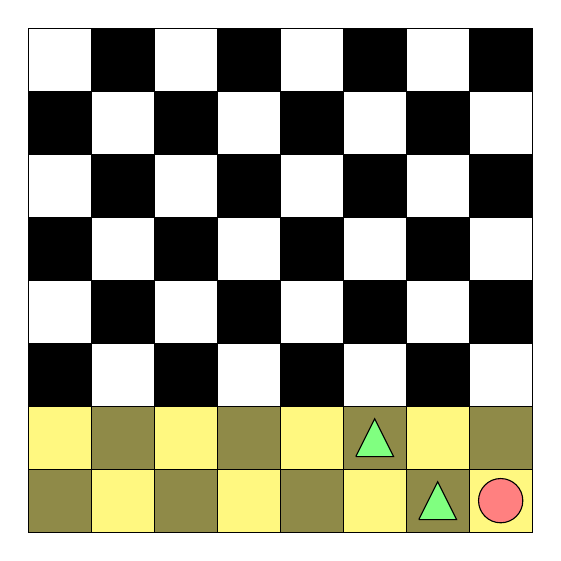
\begin{tikzpicture}
\filldraw[fill=yellow!50!black](0.8,0.8)--(1.6,0.8)--(1.6,1.6)--(0.8,1.6)--(0.8,0.8);
\filldraw[fill=yellow!50!white](0.8,1.6)--(1.6,1.6)--(1.6,2.4000000000000004)--(0.8,2.4000000000000004)--(0.8,1.6);
\filldraw[fill=black](0.8,2.4000000000000004)--(1.6,2.4000000000000004)--(1.6,3.2)--(0.8,3.2)--(0.8,2.4000000000000004);
\filldraw[fill=white](0.8,3.2)--(1.6,3.2)--(1.6,4.0)--(0.8,4.0)--(0.8,3.2);
\filldraw[fill=black](0.8,4.0)--(1.6,4.0)--(1.6,4.8)--(0.8,4.8)--(0.8,4.0);
\filldraw[fill=white](0.8,4.800000000000001)--(1.6,4.800000000000001)--(1.6,5.6000000000000005)--(0.8,5.6000000000000005)--(0.8,4.800000000000001);
\filldraw[fill=black](0.8,5.6000000000000005)--(1.6,5.6000000000000005)--(1.6,6.4)--(0.8,6.4)--(0.8,5.6000000000000005);
\filldraw[fill=white](0.8,6.4)--(1.6,6.4)--(1.6,7.2)--(0.8,7.2)--(0.8,6.4);
\filldraw[fill=yellow!50!white](1.6,0.8)--(2.4000000000000004,0.8)--(2.4000000000000004,1.6)--(1.6,1.6)--(1.6,0.8);
\filldraw[fill=yellow!50!black](1.6,1.6)--(2.4000000000000004,1.6)--(2.4000000000000004,2.4000000000000004)--(1.6,2.4000000000000004)--(1.6,1.6);
\filldraw[fill=white](1.6,2.4000000000000004)--(2.4000000000000004,2.4000000000000004)--(2.4000000000000004,3.2)--(1.6,3.2)--(1.6,2.4000000000000004);
\filldraw[fill=black](1.6,3.2)--(2.4000000000000004,3.2)--(2.4000000000000004,4.0)--(1.6,4.0)--(1.6,3.2);
\filldraw[fill=white](1.6,4.0)--(2.4000000000000004,4.0)--(2.4000000000000004,4.8)--(1.6,4.8)--(1.6,4.0);
\filldraw[fill=black](1.6,4.800000000000001)--(2.4000000000000004,4.800000000000001)--(2.4000000000000004,5.6000000000000005)--(1.6,5.6000000000000005)--(1.6,4.800000000000001);
\filldraw[fill=white](1.6,5.6000000000000005)--(2.4000000000000004,5.6000000000000005)--(2.4000000000000004,6.4)--(1.6,6.4)--(1.6,5.6000000000000005);
\filldraw[fill=black](1.6,6.4)--(2.4000000000000004,6.4)--(2.4000000000000004,7.2)--(1.6,7.2)--(1.6,6.4);
\filldraw[fill=yellow!50!black](2.4000000000000004,0.8)--(3.2,0.8)--(3.2,1.6)--(2.4000000000000004,1.6)--(2.4000000000000004,0.8);
\filldraw[fill=yellow!50!white](2.4000000000000004,1.6)--(3.2,1.6)--(3.2,2.4000000000000004)--(2.4000000000000004,2.4000000000000004)--(2.4000000000000004,1.6);
\filldraw[fill=black](2.4000000000000004,2.4000000000000004)--(3.2,2.4000000000000004)--(3.2,3.2)--(2.4000000000000004,3.2)--(2.4000000000000004,2.4000000000000004);
\filldraw[fill=white](2.4000000000000004,3.2)--(3.2,3.2)--(3.2,4.0)--(2.4000000000000004,4.0)--(2.4000000000000004,3.2);
\filldraw[fill=black](2.4000000000000004,4.0)--(3.2,4.0)--(3.2,4.8)--(2.4000000000000004,4.8)--(2.4000000000000004,4.0);
\filldraw[fill=white](2.4000000000000004,4.800000000000001)--(3.2,4.800000000000001)--(3.2,5.6000000000000005)--(2.4000000000000004,5.6000000000000005)--(2.4000000000000004,4.800000000000001);
\filldraw[fill=black](2.4000000000000004,5.6000000000000005)--(3.2,5.6000000000000005)--(3.2,6.4)--(2.4000000000000004,6.4)--(2.4000000000000004,5.6000000000000005);
\filldraw[fill=white](2.4000000000000004,6.4)--(3.2,6.4)--(3.2,7.2)--(2.4000000000000004,7.2)--(2.4000000000000004,6.4);
\filldraw[fill=yellow!50!white](3.2,0.8)--(4.0,0.8)--(4.0,1.6)--(3.2,1.6)--(3.2,0.8);
\filldraw[fill=yellow!50!black](3.2,1.6)--(4.0,1.6)--(4.0,2.4000000000000004)--(3.2,2.4000000000000004)--(3.2,1.6);
\filldraw[fill=white](3.2,2.4000000000000004)--(4.0,2.4000000000000004)--(4.0,3.2)--(3.2,3.2)--(3.2,2.4000000000000004);
\filldraw[fill=black](3.2,3.2)--(4.0,3.2)--(4.0,4.0)--(3.2,4.0)--(3.2,3.2);
\filldraw[fill=white](3.2,4.0)--(4.0,4.0)--(4.0,4.8)--(3.2,4.8)--(3.2,4.0);
\filldraw[fill=black](3.2,4.800000000000001)--(4.0,4.800000000000001)--(4.0,5.6000000000000005)--(3.2,5.6000000000000005)--(3.2,4.800000000000001);
\filldraw[fill=white](3.2,5.6000000000000005)--(4.0,5.6000000000000005)--(4.0,6.4)--(3.2,6.4)--(3.2,5.6000000000000005);
\filldraw[fill=black](3.2,6.4)--(4.0,6.4)--(4.0,7.2)--(3.2,7.2)--(3.2,6.4);
\filldraw[fill=yellow!50!black](4.0,0.8)--(4.8,0.8)--(4.8,1.6)--(4.0,1.6)--(4.0,0.8);
\filldraw[fill=yellow!50!white](4.0,1.6)--(4.8,1.6)--(4.8,2.4000000000000004)--(4.0,2.4000000000000004)--(4.0,1.6);
\filldraw[fill=black](4.0,2.4000000000000004)--(4.8,2.4000000000000004)--(4.8,3.2)--(4.0,3.2)--(4.0,2.4000000000000004);
\filldraw[fill=white](4.0,3.2)--(4.8,3.2)--(4.8,4.0)--(4.0,4.0)--(4.0,3.2);
\filldraw[fill=black](4.0,4.0)--(4.8,4.0)--(4.8,4.8)--(4.0,4.8)--(4.0,4.0);
\filldraw[fill=white](4.0,4.800000000000001)--(4.8,4.800000000000001)--(4.8,5.6000000000000005)--(4.0,5.6000000000000005)--(4.0,4.800000000000001);
\filldraw[fill=black](4.0,5.6000000000000005)--(4.8,5.6000000000000005)--(4.8,6.4)--(4.0,6.4)--(4.0,5.6000000000000005);
\filldraw[fill=white](4.0,6.4)--(4.8,6.4)--(4.8,7.2)--(4.0,7.2)--(4.0,6.4);
\filldraw[fill=yellow!50!white](4.800000000000001,0.8)--(5.6000000000000005,0.8)--(5.6000000000000005,1.6)--(4.800000000000001,1.6)--(4.800000000000001,0.8);
\filldraw[fill=yellow!50!black](4.800000000000001,1.6)--(5.6000000000000005,1.6)--(5.6000000000000005,2.4000000000000004)--(4.800000000000001,2.4000000000000004)--(4.800000000000001,1.6);
\filldraw[fill=green!50!white] (4.960000000000001,1.7600000000000002)--(5.44,1.7600000000000002)--(5.2,2.2399999999999998)--(4.960000000000001,1.7600000000000002);
\filldraw[fill=white](4.800000000000001,2.4000000000000004)--(5.6000000000000005,2.4000000000000004)--(5.6000000000000005,3.2)--(4.800000000000001,3.2)--(4.800000000000001,2.4000000000000004);
\filldraw[fill=black](4.800000000000001,3.2)--(5.6000000000000005,3.2)--(5.6000000000000005,4.0)--(4.800000000000001,4.0)--(4.800000000000001,3.2);
\filldraw[fill=white](4.800000000000001,4.0)--(5.6000000000000005,4.0)--(5.6000000000000005,4.8)--(4.800000000000001,4.8)--(4.800000000000001,4.0);
\filldraw[fill=black](4.800000000000001,4.800000000000001)--(5.6000000000000005,4.800000000000001)--(5.6000000000000005,5.6000000000000005)--(4.800000000000001,5.6000000000000005)--(4.800000000000001,4.800000000000001);
\filldraw[fill=white](4.800000000000001,5.6000000000000005)--(5.6000000000000005,5.6000000000000005)--(5.6000000000000005,6.4)--(4.800000000000001,6.4)--(4.800000000000001,5.6000000000000005);
\filldraw[fill=black](4.800000000000001,6.4)--(5.6000000000000005,6.4)--(5.6000000000000005,7.2)--(4.800000000000001,7.2)--(4.800000000000001,6.4);
\filldraw[fill=yellow!50!black](5.6000000000000005,0.8)--(6.4,0.8)--(6.4,1.6)--(5.6000000000000005,1.6)--(5.6000000000000005,0.8);
\filldraw[fill=green!50!white] (5.760000000000001,0.96)--(6.24,0.96)--(6.0,1.4400000000000002)--(5.760000000000001,0.96);
\filldraw[fill=yellow!50!white](5.6000000000000005,1.6)--(6.4,1.6)--(6.4,2.4000000000000004)--(5.6000000000000005,2.4000000000000004)--(5.6000000000000005,1.6);
\filldraw[fill=black](5.6000000000000005,2.4000000000000004)--(6.4,2.4000000000000004)--(6.4,3.2)--(5.6000000000000005,3.2)--(5.6000000000000005,2.4000000000000004);
\filldraw[fill=white](5.6000000000000005,3.2)--(6.4,3.2)--(6.4,4.0)--(5.6000000000000005,4.0)--(5.6000000000000005,3.2);
\filldraw[fill=black](5.6000000000000005,4.0)--(6.4,4.0)--(6.4,4.8)--(5.6000000000000005,4.8)--(5.6000000000000005,4.0);
\filldraw[fill=white](5.6000000000000005,4.800000000000001)--(6.4,4.800000000000001)--(6.4,5.6000000000000005)--(5.6000000000000005,5.6000000000000005)--(5.6000000000000005,4.800000000000001);
\filldraw[fill=black](5.6000000000000005,5.6000000000000005)--(6.4,5.6000000000000005)--(6.4,6.4)--(5.6000000000000005,6.4)--(5.6000000000000005,5.6000000000000005);
\filldraw[fill=white](5.6000000000000005,6.4)--(6.4,6.4)--(6.4,7.2)--(5.6000000000000005,7.2)--(5.6000000000000005,6.4);
\filldraw[fill=yellow!50!white](6.4,0.8)--(7.2,0.8)--(7.2,1.6)--(6.4,1.6)--(6.4,0.8);
\filldraw[fill=red!50!white] (6.800000000000001,1.2000000000000002) circle (8pt);
\filldraw[fill=yellow!50!black](6.4,1.6)--(7.2,1.6)--(7.2,2.4000000000000004)--(6.4,2.4000000000000004)--(6.4,1.6);
\filldraw[fill=white](6.4,2.4000000000000004)--(7.2,2.4000000000000004)--(7.2,3.2)--(6.4,3.2)--(6.4,2.4000000000000004);
\filldraw[fill=black](6.4,3.2)--(7.2,3.2)--(7.2,4.0)--(6.4,4.0)--(6.4,3.2);
\filldraw[fill=white](6.4,4.0)--(7.2,4.0)--(7.2,4.8)--(6.4,4.8)--(6.4,4.0);
\filldraw[fill=black](6.4,4.800000000000001)--(7.2,4.800000000000001)--(7.2,5.6000000000000005)--(6.4,5.6000000000000005)--(6.4,4.800000000000001);
\filldraw[fill=white](6.4,5.6000000000000005)--(7.2,5.6000000000000005)--(7.2,6.4)--(6.4,6.4)--(6.4,5.6000000000000005);
\filldraw[fill=black](6.4,6.4)--(7.2,6.4)--(7.2,7.2)--(6.4,7.2)--(6.4,6.4);
\end{tikzpicture}
\caption{
حالت هایی که به مات شدن منجر نمی شوند.
}
\end{figure}

\newpage

\Q

هر مجموعه‌ی $n$ عضوی، 
$
2^n
$
زیرمجموعه دارد. ابتدا یکی از زیرمجموعه‌های 
$
k
$
عضوی را به تصادف بر می‌داریم. این کار به 
$
\binom{n}{k}
$
طریق امکان دارد. برای آن که زیرمجموعه‌ی دیگر، با زیرمجموعه‌ی انتخاب شده ناسازگار باشد، باید اعضای آن از بین 
$
n-k
$
عضو باقیمانده به 
$
2^{n-k}
$
طریق ممکن انتخاب شوند. در نتیجه تعداد حالات مطلوب (برای هر زیرمجموعه با هر تعداد عضو)، طبق اصل ضرب برابر
$
\sum_{k=0}^n\binom{n}{k}2^{n-k}
$
خواهد بود. با این حال، باید دقت شود که تعدادی از حالات تکراری اند. به طور مثال، امکان دارد زیرمجموعه‌ی 
$
\{1,3,n\}
$
، در دفعه‌ی اول و زیرمجموعه‌ی 
$
\{2,4,n-1\}
$
در دفعه‌ی دوم از بین اعضای باقیمانده انتخاب شود؛ یا بالعکس. همچنین، حالتی که هر دو زیرمجموعه تهی باشند، شمرده شده است که با وجود ناسازگاری، متمایز نیستند. پس باید از تعداد کل حالات مطلوب کنار گذاشته شوند. در نتیجه، حالات مطلوب برداشتن دو زیرمجموعه‌ی ناسازگار متمایز، برابر
$
\frac{
[\sum_{k=0}^n\binom{n}{k}2^{n-k}]-1
}{2}
$
و احتمال مطلوب، برابر
$
\frac{
\frac{
[\sum_{k=0}^n\binom{n}{k}2^{n-k}]-1
}{2}
}{
\binom{2^n}{2}
}
$
خواهد بود.

(با ساده سازی، می توان احتمال را به صورت زیر نیز نوشت
$$
\frac{
3^n-1
}{
2^n(2^n-1)
}
$$
)

\end{document}